\cleardoublepage
\chapter{Impurity levels of point defects\label{ch:defects}}
In this chapter, we present the preliminary study of defect levels in semiconductors with Koopmans spectral functionals. 

\clearpage
\section{Motivation\label{sec:motivation-defects}}
Many properties of materials are strongly influenced by the presence of impurities and point defects. Electrical and optical properties of semiconductors can be both quenched and stimulated as a consequence of the presence of defects. In extrinsic semiconductors, the hole and electron conductivities can be finely controlled by tuning the concentration of $p$-type impurity atoms -- also called acceptors, as they trap an electron and free a hole close to the top of the valence band -- and $n$-type impurity atoms -- also called donors, as they release an electron at the bottom of the conduction band. On the other hand, the presence of defect centers can also have a reversed effect and trap charge carriers in localized states, as for gold impurities in silicon \cite{corsetti_negative-u_2014}, decreasing the conductivity of the material. More recently, the properties of impurity centers have been considered also in the context of quantum information, since they can represent optimal systems for quantum communication: the infamous nitrogen-vacancy (NV) center in diamond is one of them \cite{maze_properties_2011}, as it provides a very coherent optical transition that can be exploited to create an entangled state (a qubit of information). It is apparent, that many modern electronic and optoelectronic devices, are somehow affected by the presence of defects -- negatively, or positively. Understanding, and being able to properly simulate such effects, is then an extremely relevant topic in computational materials science.

To test the performances of Koopmans functionals for the prediction of the position of impurity levels in semiconductors, we considered the EL2 defect in gallium arsenide. The EL2 defect has been for many years a pivotal research topic due to its influence on the electrical and optical properties of GaAs, and for its appearance during the growth process of melt GaAs, despite the total absence of any doping elements. It was observed experimentally that the EL2 concentration increases with the stoichiometry ratio of the elemental species As/Ga \cite{kaminska_el2_1987}, which hinted at a connection with the As atom. Whether the EL2 defect is associated with a substitutional As-antisite -- taking the place of a Ga vacancy -- or with a complex of As-antisite with As-interstitial, was object of debate for a while; today, the interpretation of the simple As-antisite ($\asga$) impurity is commonly accepted. The EL2 defect level is then given by the presence of a neutral As-antisite and lies 0.75~\mev below the bottom of the conduction band \cite{kaminska_el2_1987,dabrowski_isolated_1989}. The positively charged state ($\rm As_{Ga}^+$) lies instead 0.5~\mev above the top of the valence band. Given the simple nature of this defect -- the neutral As-antisite defect state is a fully symmetric ($A_1$) singlet -- and the excellent description of the band structure of GaAs from Koopmans functionals (see \cref{ch:band-structures}), the $\asga$ represents a perfect test case.

\section{Theoretical schemes\label{sec:theory-defects}}
In a mean-field approach, the Schr\"{o}dinger equation of a crystalline material whose translation symmetry is broken by the presence of some point defect (substitutional or interstitial atoms, vacancies, dislocations, etc.) reads as
%
\begin{equation}
    -\frac{1}{2} \nabla^2 \psi + \big( V + U_{\rm d } \big) \psi = E \psi ,
    \label{eq:schrodinger-eq-defects}
\end{equation}
%
where $V$ is the periodic crystal potential, and $U_{\rm d}$ is the potential due to the presence of the impurity. Depending on the spatial extension of the wave function $\psi$, two different regimes can be identified. When the wave function spreads over the lattice, the potential $U_{\rm d}$ is much smaller than the crystal potential, thus can be treated as a small perturbation; this is the case of \emph{shallow} impurity states. Instead, when $\psi$ is localized in a small region surrounding the point defect, the impurity potential becomes dominant in that region and is the crystal potential that can be treated perturbatively; this is the case of \emph{deep} -- tightly bound -- defect states. The energy levels arising within the material's band gap, upon the formation of a shallow defect state, are usually located very close to the band edges, whereas the levels associated to deep states are much more bound and sit around mid-gap.

\begin{figure}
    \centering
    \subfloat[]{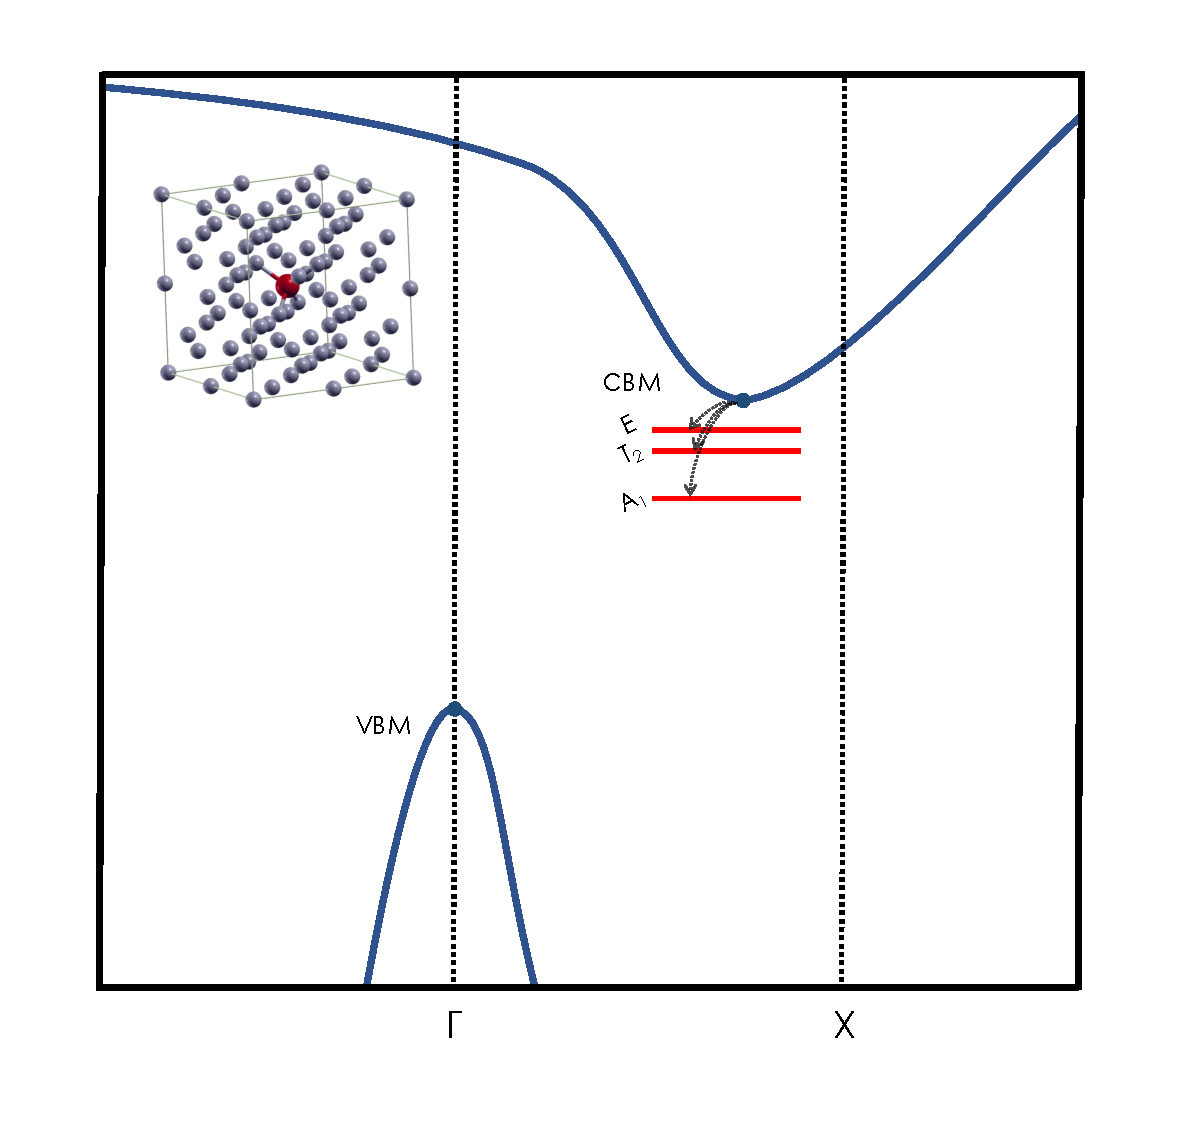
\includegraphics[width=.5\linewidth]{as-si-levels.pdf}}
    \subfloat[]{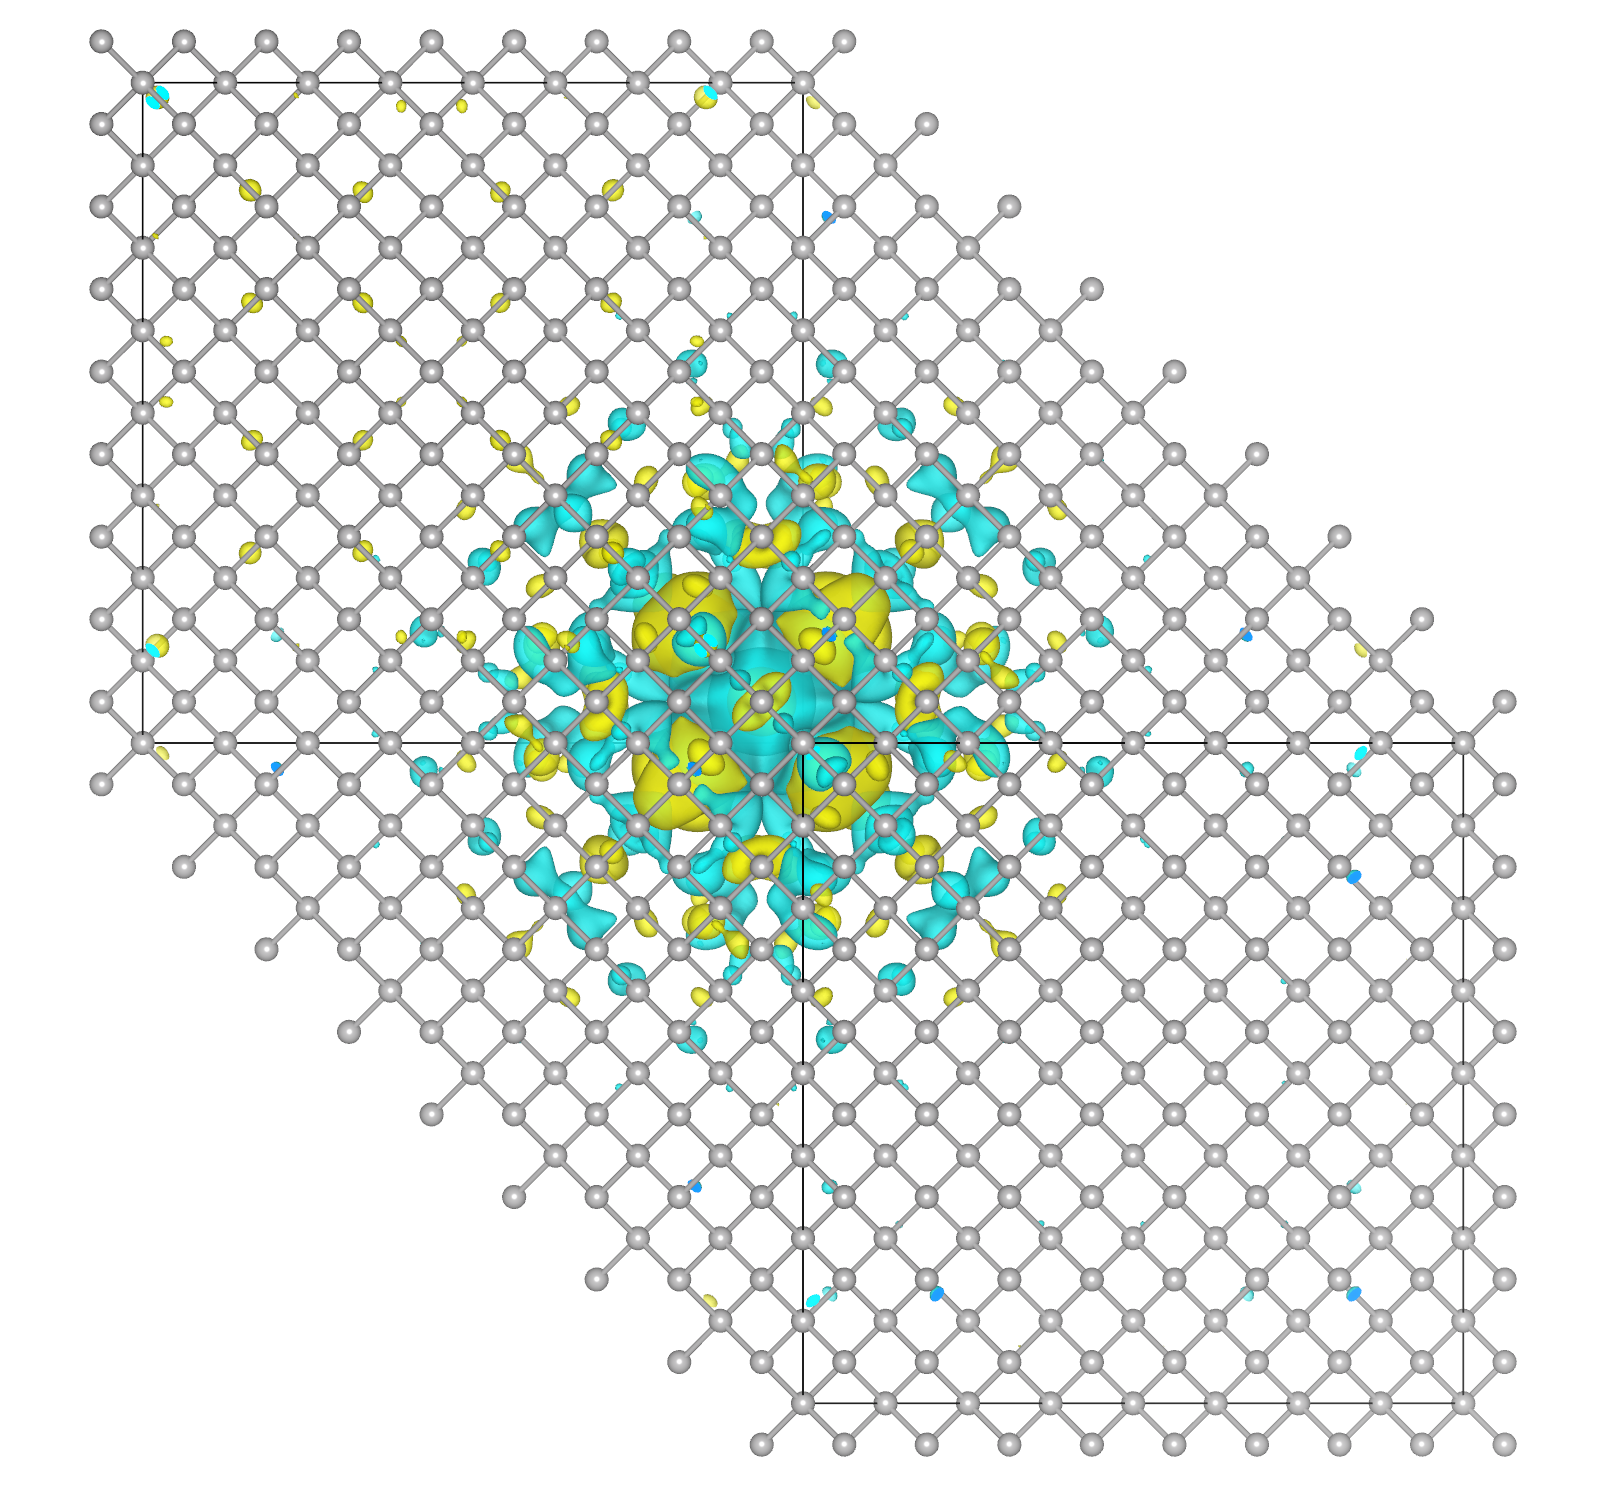
\includegraphics[width=.5\linewidth]{defect_wfc_888.png}}
    \caption[]{Impurity states emerging in As-doped silicon. On the left, we show the three shallow energy levels forming within the band gap: a singlet ($A_1$) at 53.8~\mev below the conduction band minimum, a triplet ($T_2$) at 32.7~\mev, and a doublet ($E$) at 31.3~\mev. On the right, we show an isosurface of the orbital density of the $A_1$ defect state in a supercell containing 1024 atoms.}
    \label{fig:as-si-defect}
\end{figure}

For shallow impurities ($U_{\rm d} \ll V$), the zeroth-order Hamiltonian is that of the pristine material, therefore it is natural to represent the electronic states with Bloch functions. Historically, this type of impurities have been studied by means of the effective-mass equation, and in the Kohn-Luttinger formulation \cite{kohn_theory_1955} -- where $U_{\rm d}$ is modeled via a dielectrically screened Coulomb potential -- the predictions of the shallow donor states of silicon are in good agreement with the experiment. One of the issues with the effective-mass equation is that it totally misses the level splitting due to the breaking of the point symmetry of the unit cell (caused by the presence of the impurity). If we consider for instance As-doped Si, the symmetry passes from $O_h$ to the smaller group $T_d$, and the six-fold degenerate conduction band minimum (CBM) splits into three groups of levels (as showed in \cref{fig:as-si-defect}). First-principles methods usually embody all the symmetries of the system, and indeed the spectrum obtained, e.g., at the DFT level, predicts the correct splitting of the energy levels. Problem is that the size of the supercell required to contain the density of a shallow defect state, can rapidly become unfeasible -- in As-doped Si it was showed that DFT results converge only for about $10^4$-atom supercells \cite{yamamoto_first-principles_2009}. For such systems, DFT represents the only possible first-principles approach, however, the intrinsic incapability of describing the electronic energies via the KS eigenvalues, demands for higher-level methods. Besides, it is worth to mention that schemes that include \emph{a posteriori} corrections of the KS eigenvalues, showed a remarkable accuracy in the prediction of the shallow donor states of silicon \cite{yamamoto_first-principles_2009,smith_ab_2017}.

Deep defect states are instead more easy to tackle from a computational point of view. The dominant character of the impurity potential ($U_{\rm d} \gg V$) in the region of the defect center, favors the localization of the wave function. The supercells used to model this type of defects contain an order of $10^2$ atoms, which makes calculations with advanced electronic-structure methods more feasible. In the following we report two possible approaches to the problem, based on hybrid functionals and Green's function theory, and see how those can be employed in the context of Koopmans functionals.

\subsection{The formation energy approach}

\subsection{The quasiparticle approach}

\section{Results and discussions}





